\section{Testen}

Het is belangrijk dat bepaalde eigenschappen van de gemaakte sensormodule goed getest worden. In dit hoofdstuk worden vier tests beschreven die zijn gedaan om te bepalen of de sensormodule goed functioneert. Bij elke test staat een tabel met materialen die gebruikt zijn. Na de beschrijving van elke test worden de resultaten getoond, gevolgd door een discussie over deze resultaten.


\subsection{Stabiliteitstest}\label{sec:stabiliteitstest}
De eerste test is bedoelt om te controleren of de uitgang van de opamp stabiel is. Dit is een belangrijke test om uit te voeren; als de uitgang niet stabiel is, zal de spanning die de ADC uitleest niet goed overeen komen met de drempelspanning van de ISFET.
Bij deze test zijn de materialen uit \cref{tab:testMaterialen1} gebruikt.
\begin{table}[!htbp]
    \centering
    \begin{tabular}{l|l|l}
        Apparaat         & Serienummer & Beschrijving \\
        \hline
        MSREF1           & 23/RS03     & Referentie elektrode       \\
        MSFET 3330-2     & 23/205      & ISFET pH sensor            \\
        Tektronix MSO 46 & C019070     & Oscilloscoop               \\
        Uitlees PCB      & 1           & ISFET uitlees schakeling   \\
        Voeding PCB      & 1           & BMS en energy harvester    \\
        \hline
    \end{tabular}
    \caption{De materialen die zijn gebruikt voor de stabiliteitstest.}
    \label{tab:testMaterialen1}
\end{table}

Om de test uit te voeren wordt de uitlees PCB verbonden met de voeding PCB, zodat de uitleesschakeling een voeding heeft. De probe van kanaal 1 van de oscilloscoop wordt verbonden met de uitgang van de opamp. De probe van kanaal 2 wordt verbonden met de drain van de ISFET. De ISFET wordt samen met de referentieelektrode in een pH 7 bufferoplossing gestopt. De opstelling is in \cref{fig:test ISFET circuit best} schematisch te zien.

\begin{figure}[!htbp]
    \centering
    \def\svgwidth{0.75\textwidth}
    \input{img/ISFETCircuitBestTest.pdf_tex}
    \caption{De locatie van de scope probes in de schakeling om te testen of de uitgang stabiel is.}
    \label{fig:test ISFET circuit best}
\end{figure}


\subsubsection{Resultaten van de stabiliteitstest} \label{sec:stabilityTestResults}

De eerste test resulteerde in een oscillerend signaal. De uitgang van de opamp gaf een signaal dat elke \qty{6.8}{\milli\second} pulseerde. Dit is te zien in \cref{fig:resultUgsUds}.
Wanneer de opamp uitgang laag is, waardoor de gate-source spanning op de ISFET \qty{0}{\volt} wordt, komt de drain-source spanning van de ISFET erg langzaam omhoog. Wanneer deze spanning boven de referentiespanning komt, gaat de uitgang van de opamp omhoog, waarna de drain-source spanning van de ISFET erg snel begint te dalen. Echter, wanneer de drain-source spanning vervolgens de referentiespanning bereikt, reageert de opamp hier merkwaardig genoeg niet direct op. Dit zorgt voor een oscillerende werking. Ditzelfde resultaat kwam uit dezelfde test met een andere opmamp (de MCP6002).

Op de drain-source spanning is ook een tweede oscillatie met een hogere frequentie zichtbaar.


% Een mogelijke reden hiervoor is dat de ISFET niet snel genoeg reageert op spanningsveranderingen tussen de gate (de referentie elektrode) en de source.

%

% Dit wordt waarschijnlijk veroorzaakt door de interne chopping van de gekozen opamp.

\begin{figure}[!htbp]
    \centering
    \def\svgwidth{0.75\textwidth}
    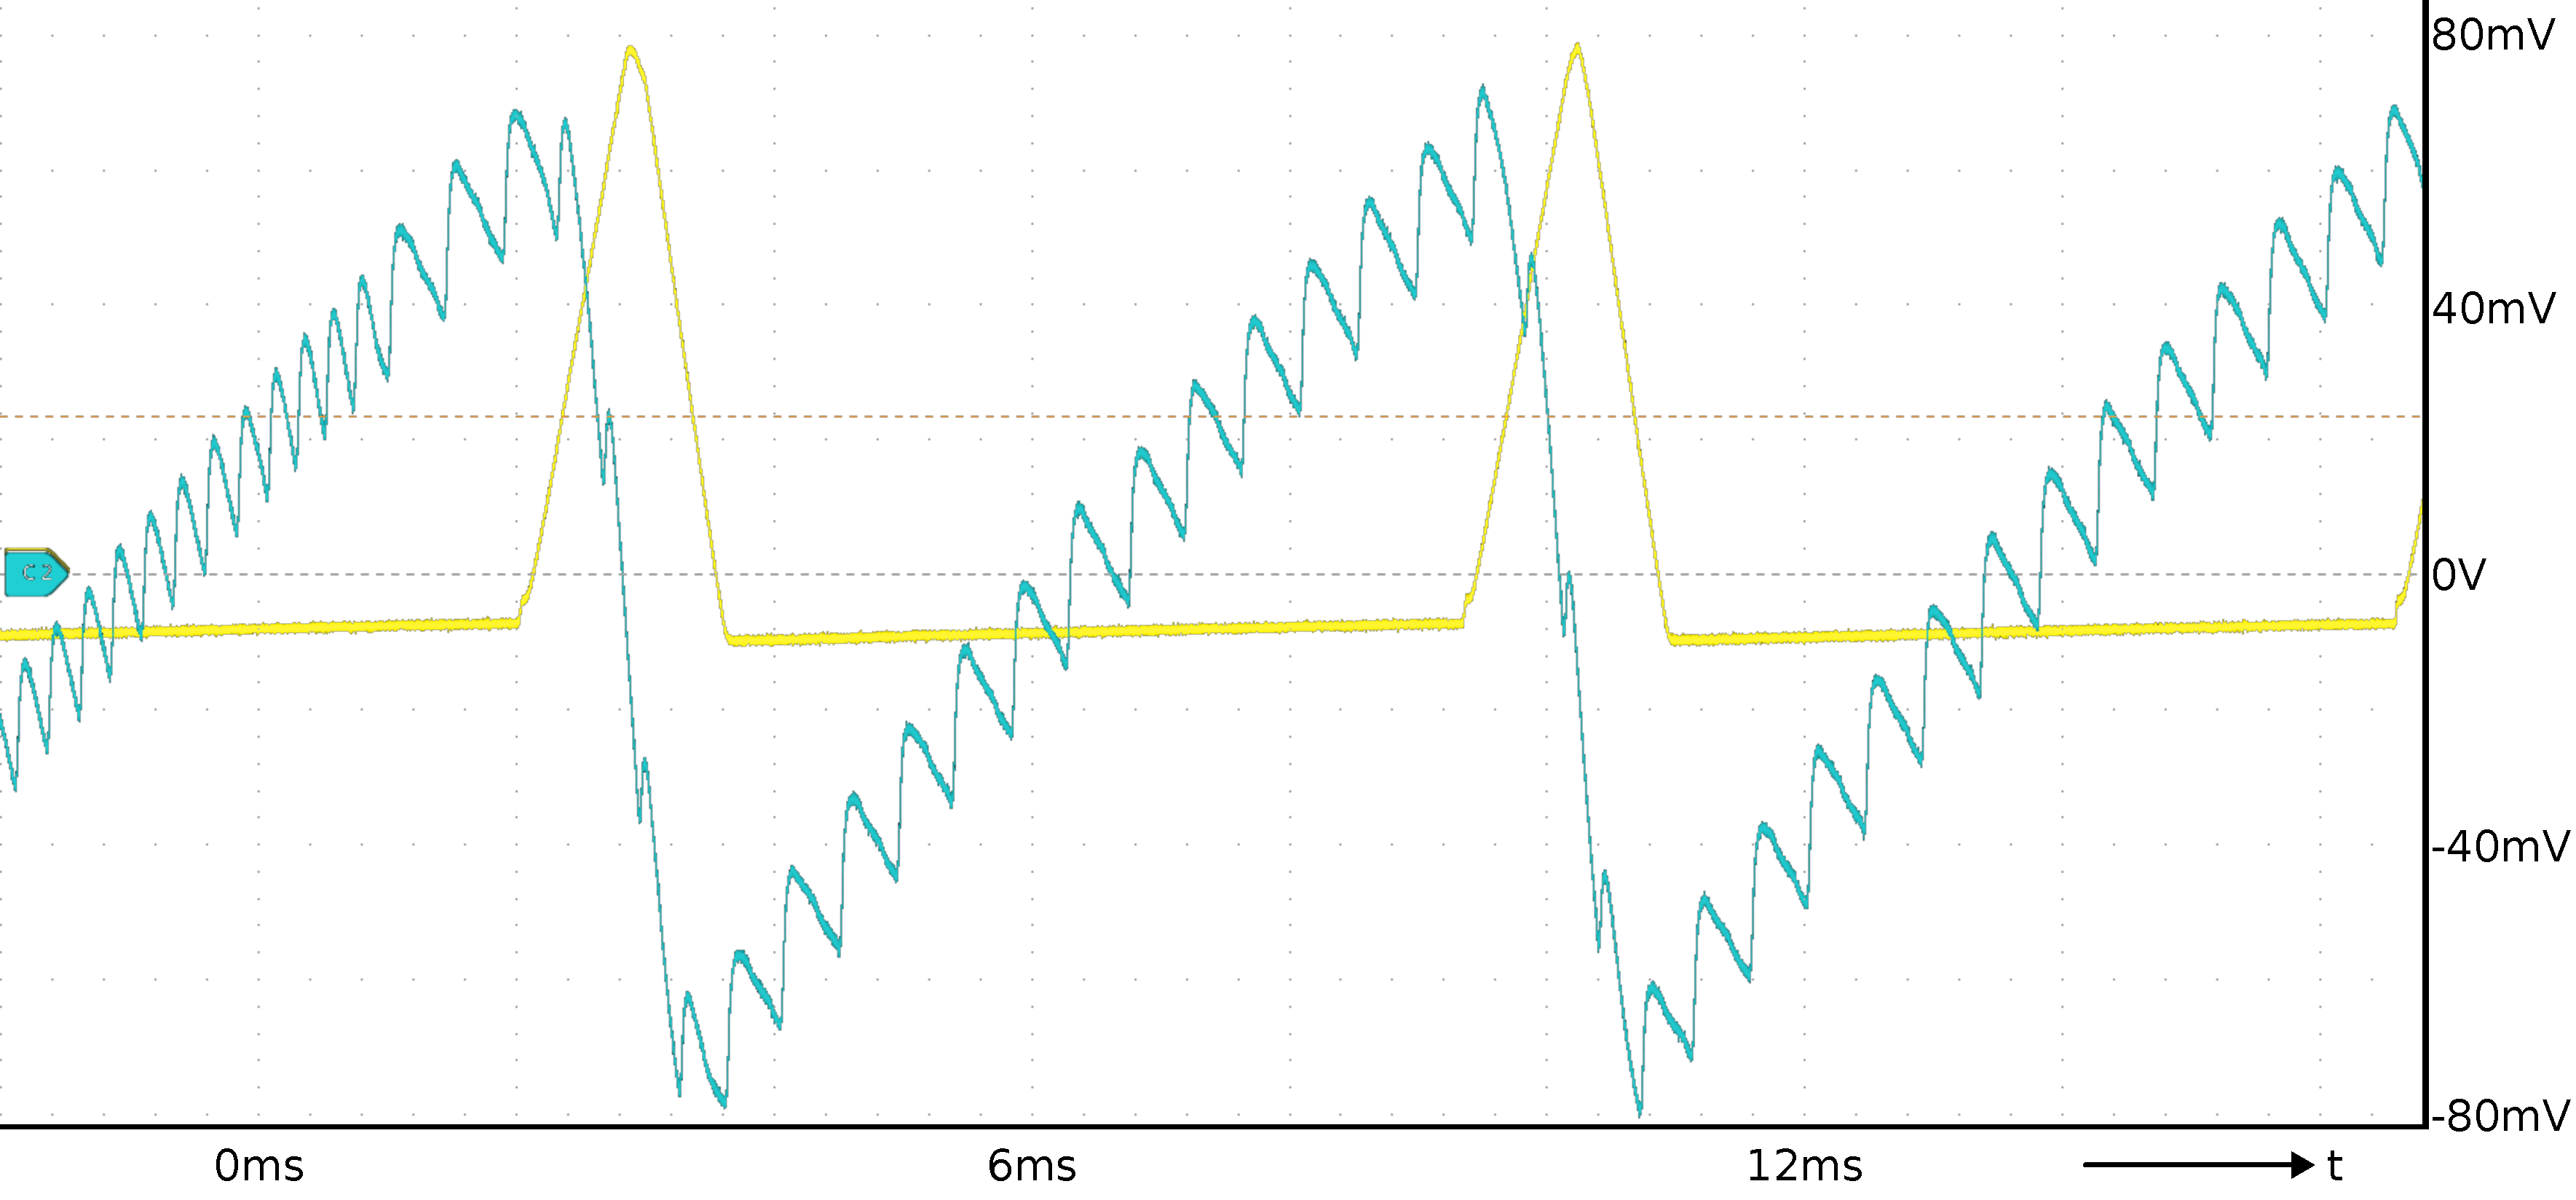
\includegraphics[width=\textwidth]{testUgsUds.pdf}
    \caption{Het resultaat van de stabiliteitstest. De x-as is tijd, de y-as is spanning. Kanaal 1 (geel) is $U_{gs}$, kanaal 2 (lichtblauw) is $U_{ds}$.}
    \label{fig:resultUgsUds}
\end{figure}


\subsubsection{Discussie van de stabiliteitstest}
Er zijn meerdere mogelijke oplossingen voor de instabiliteit.
Eén mogelijke oplossing is een integrator plaatsen tussen de uitgang van de opamp en de gate van de ISFET. Dit zou ervoor zorgen dat de ISFET genoeg tijd heeft om te reageren op de veranderde gate-source spanning, waardoor deze de opamp kan bijhouden.

Een andere mogelijke oplossing is een RC-filter te plaatsen tussen de drain van de ISFET en de niet-inverterende ingang van de opamp. Dit zorgt ervoor dat de opamp trager gaat werken, waardoor de ISFET de opamp bij kan houden.

Er zal een aantal tests gedaan moeten worden om te vinden hoe de ISFET precies reageert op een verandering van de gate-source spanning, en hoe dit verschilt van een reguliere MOSFET. Zo kan een beter model opgesteld worden van de ISFET, waar dan vervolgens een betere uitleesschakeling mee ontworpen kan worden.


\subsection{pH waarde test}
Deze test is bedoelt om te testen of het uitgangssignaal verandert op basis van de pH waarde. Voor deze test zijn de materialen uit \cref{tab:testMaterialen2} gebruikt.
\begin{table}[!htbp]
    \centering
    \begin{tabular}{l|l|l}
        Apparaat         & Serienummer & Beschrijving \\
        \hline
        MSREF1           & 23/RS03     & Referentie elektrode       \\
        MSFET 3330-2     & 23/205      & ISFET pH sensor            \\
        Tektronix MSO 46 & C019070     & Oscilloscoop               \\
        Uitlees PCB      & 1           & ISFET uitlees schakeling   \\
        Voeding PCB      & 1           & BMS en energy harvester    \\
        \hline
    \end{tabular}
    \caption{De materialen die zijn gebruikt voor de pH waarde test.}
    \label{tab:testMaterialen2}
\end{table}

Om te beginnen wordt de uitlees PCB verbonden met de voeding PCB, zodat de uitleesschakeling gevoed wordt. De probe van kanaal 1 van de oscilloscoop wordt verbonden met de ingang van de ADC. De probe van kanaal 2 wordt verbonden met de uitgang van de opamp. Vervolgens worden de ISFET en referentieelektrode in een pH 7 bufferoplossing gestopt. De golfvorm die de oscilloscoop geeft kan nu worden opgeslagen. De meting wordt herhaalt met de ISFET en referentieelektrode in een pH 4 bufferoplossing.

\subsubsection{Resultaten van de pH waarde test}
De resultaten van deze test zijn te zien in \cref{fig:resultspHMeasure}. Duidelijk is de amplitude van de uitgang van de opamp hoger op pH 7 vergeleken met pH 4.

\begin{figure}[!htbp]
    \centering
    \begin{subfigure}[b]{0.49\textwidth}
        \centering
        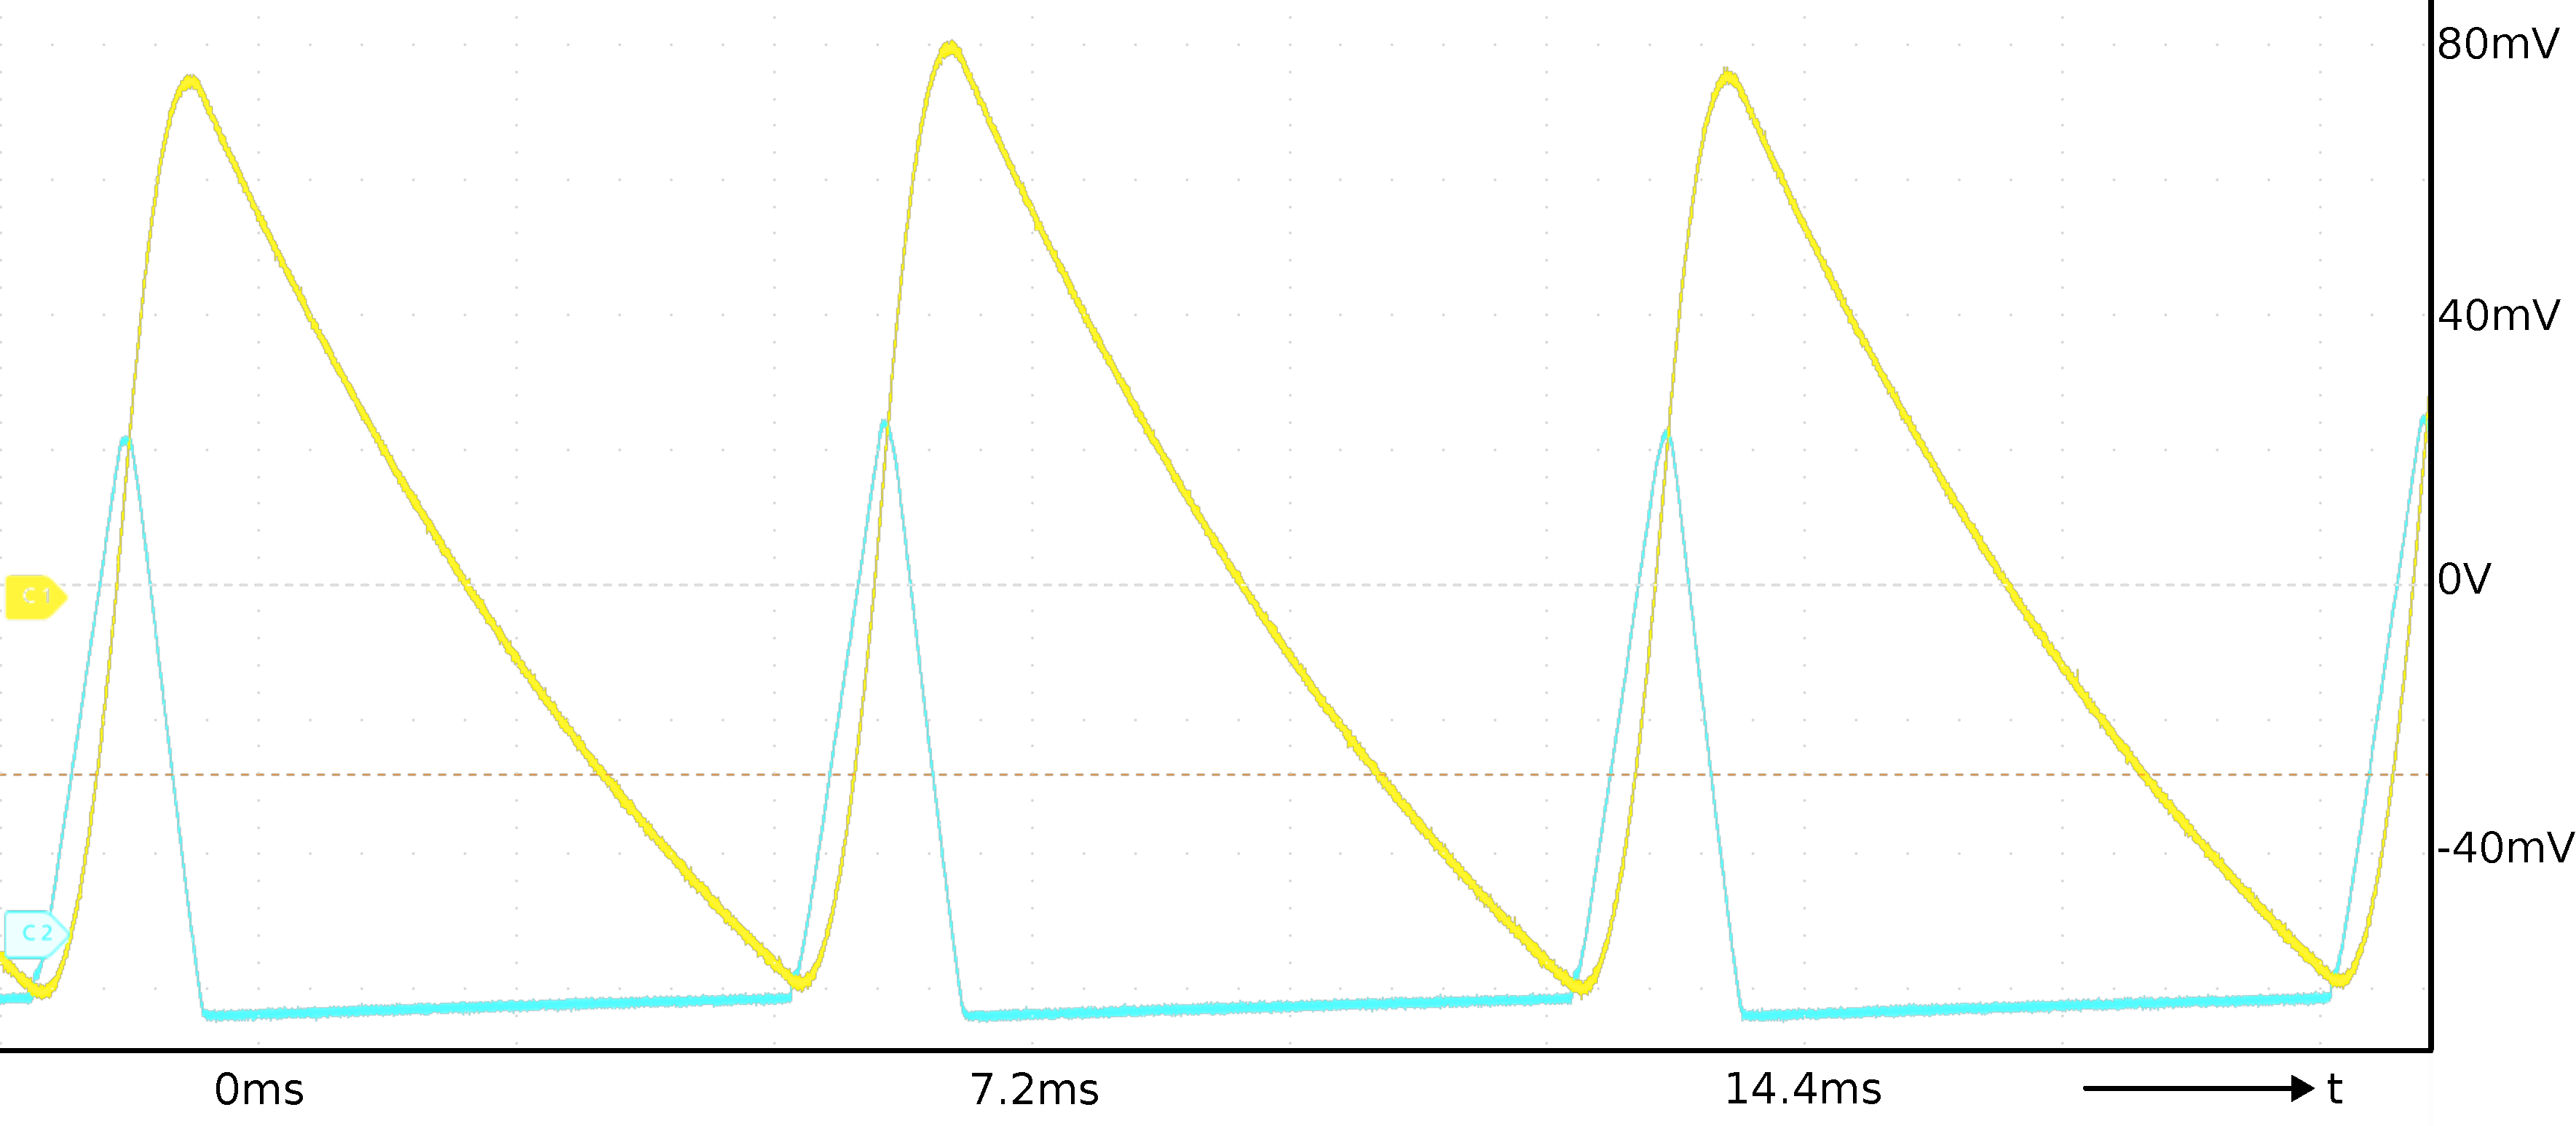
\includegraphics[width=\textwidth]{testpH7.pdf}
        \caption{De uitgang van de opamp (lichtblauw) en ingang van de ADC (geel) op pH 7.}
        \label{fig:resultpH7}
    \end{subfigure}
    \hfill
    \begin{subfigure}[b]{0.49\textwidth}
        \centering
        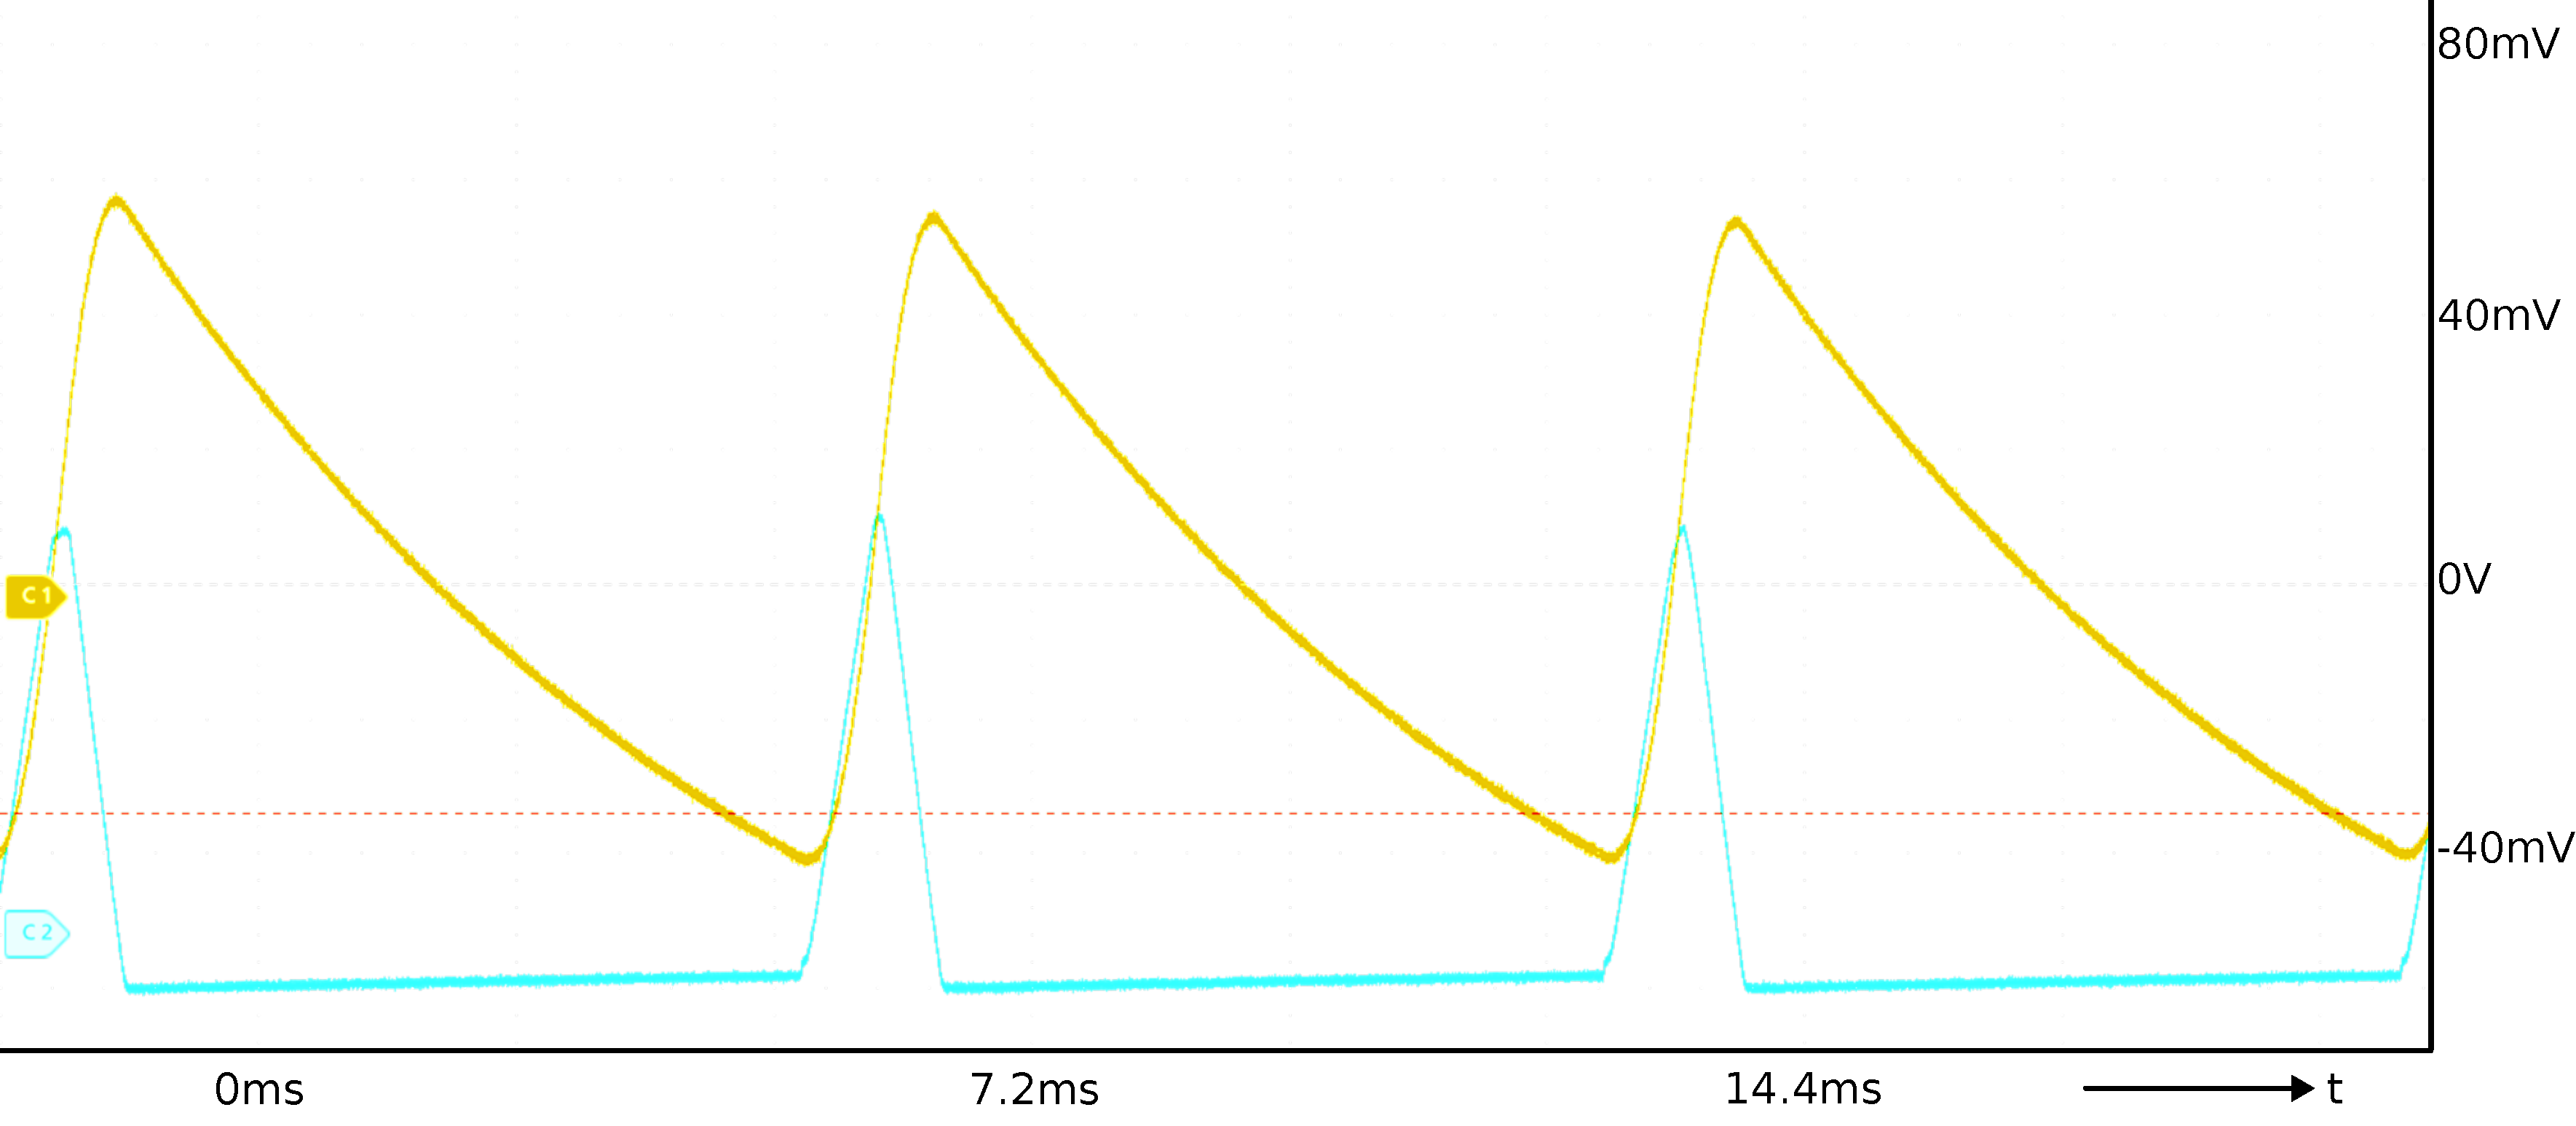
\includegraphics[width=\textwidth]{testpH4.pdf}
        \caption{De uitgang van de opamp (lichtblauw) en ingang van de ADC (geel) op pH 4.}
        \label{fig:resultpH4}
    \end{subfigure}
    \caption{De uitgang van de meetschakeling op pH 4 en pH 7. Beide metingen hebben dezelfde schaal. De x-assen zijn tijd, de y-assen zijn spanning.I've }
    \label{fig:resultspHMeasure}
\end{figure}

\subsubsection{Discussie van de pH waarde test}
Een verandering van pH waarde heeft duidelijk een effect op het uitgangssignaal. Er kan echter nog weinig gezegd worden over de lineariteit van de uitgang op basis van de pH waarde. Hiervoor zou de uitgang eerst stabiel gemaakt moeten worden.




\subsection{Vermogen test} \label{sec:vermogenTest}
Deze test is bedoelt om te controleren of het volledige systeem minder dan 10 mW aan vermogen gebruikt. Dit is gedaan door te de batterijspanning en -stroom te meten terwijl het systeem de pH waarde van een oplossing meet en opstuurt. De materialen die voor deze test zijn gebruikt zijn te vinden in \cref{tab:testMaterialen3}.
\begin{table}[!htbp]
    \centering
    \begin{tabular}{l|l|l}
        Apparaat         & Serienummer & Beschrijving \\
        \hline
        MSREF1           & 23/RS03     & Referentie elektrode       \\
        MSFET 3330-2     & 23/205      & ISFET pH sensor            \\
        Uitlees PCB      & 1           & ISFET uitlees schakeling   \\
        Voeding PCB      & 1           & BMS en energy harvester    \\
        Keithley DMM6500 & 04458071    & Multimeter spanningsmeting \\
        Keithley DMM6500 & 04458625    & Multimeter stroommeting    \\
        \hline
    \end{tabular}
    \caption{De materialen die zijn gebruikt voor de vermogen test.}
    \label{tab:testMaterialen3}
\end{table}
De opstelling staat uitgebeeld in \cref{fig:vermogenMetingOpstelling}. Eén van de twee Keithley multimeters, Scope 1 in \cref{fig:vermogenMetingOpstelling}, meet de stroom die vanuit de batterij het systeem ingaat. De andere Keit hley multimeter meet de spanning over de accu.


\begin{figure}[!htbp]
    \centering
    \def\svgwidth{0.6\textwidth}
    \input{img/vermogenTest.pdf_tex}
    \caption{Vermogen meting van systeem}
    \label{fig:vermogenMetingOpstelling}
\end{figure}

\subsubsection{Resultaten van de vermogen test}
De gemeten batterijspanning was \qty{3.82}{\volt}, tijdens de loop van de test was deze constant. Het stroomverbruik is tijdens het normaal functioneren van het systeem gemeten tussen \qty{1.3}{\milli\ampere} en \qty{2.5}{\milli\ampere}. De gemeten stroomwaardes zijn vermenigvuldigd met \qty{3.82}{\volt} en vervolgens geplot. Deze plot is te zien in \cref{fig:vermogenMeting}. Door het gemiddelde te nemen van alle samples is er een gemiddeld vermogen uitgerekend, die uitkwam op \qty{6.81}{\milli\watt}.

\begin{figure}[!htbp]
    \centering
    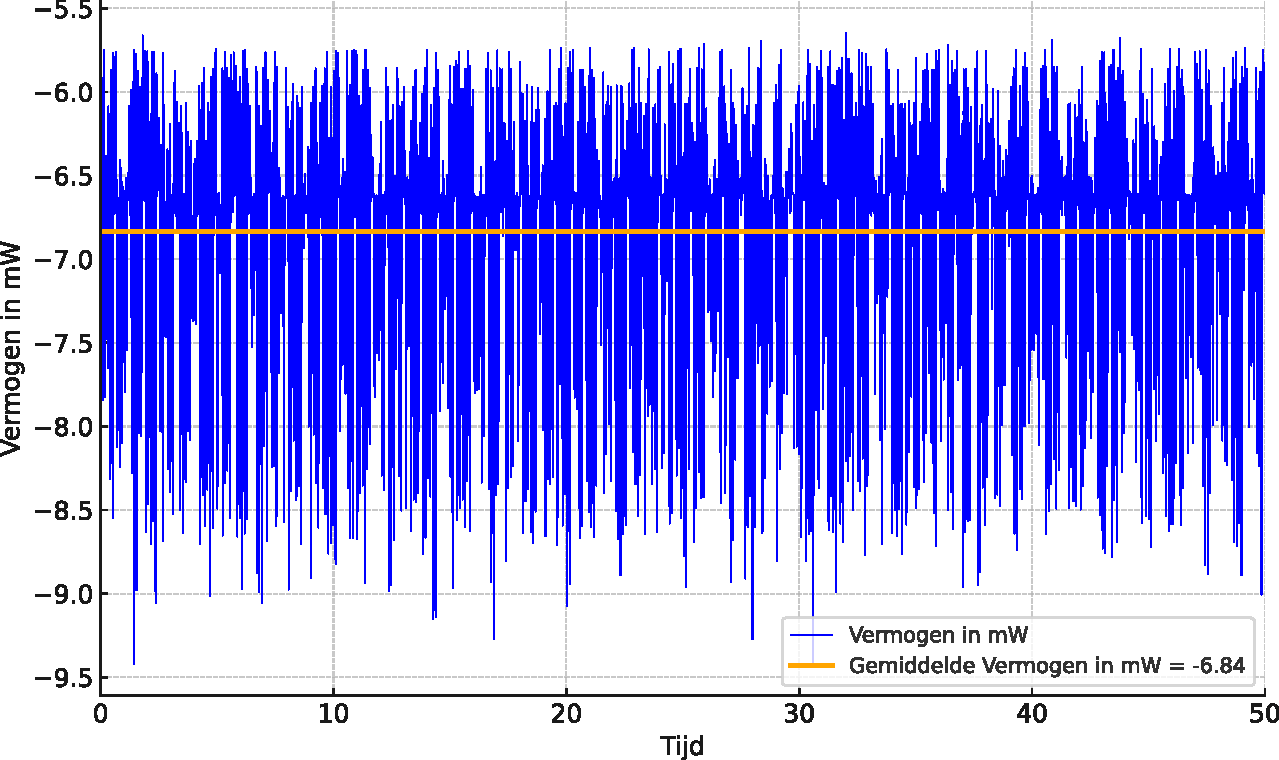
\includegraphics[width=.85\textwidth]{img/vermogensMeting.pdf}
    \caption{Vermogen meting van systeem}
    \label{fig:vermogenMeting}
\end{figure}

\subsubsection{Discussie van de vermogen test}
Uit de metingen is duidelijk te zien dat het hele systeem minder vermogen verbruikt dan de maximale \qty{10}{\milli\watt} die genoemd is in de \cref{sec:systemSpecifications}. Het energiebudget is dus behaald.


\subsection{Energy harvesting test}
Deze test is bedoelt om te meten of het energy harvesting systeem daadwerkelijk energie kan opwekken. Deze test gebruikt de materialen uit \cref{tab:testMaterialen4}.

\begin{table}[!htbp]
    \centering
    \begin{tabular}{l|l|l}
        Apparaat         & Serienummer & Beschrijving \\
        \hline
        Voeding PCB      & 1           & BMS en energy harvester    \\
        Keithley DMM6500 & 04458071    & Multimeter spanningsmeting \\
        Keithley DMM6500 & 04458625    & Multimeter stroommeting    \\
        \hline
    \end{tabular}
    \caption{De materialen die zijn gebruikt voor de energy harvesting test.}
    \label{tab:testMaterialen4}
\end{table}

De twee Keithley multimeters zijn aangesloten op dezelfde manier als in \cref{sec:vermogenTest}. Het piëzo element is door middel van een magneet een boormachine kop vastgemaakt. Dit zorgt ervoor dat het piëzo-element trilt bij het draaien van de boormachine. Het piëzo element is vervolgens aangesloten op de voeding PCB, zodat deze energie kan leveren aan het systeem en de accu. Bij deze test is alleen de voeding PCB aanwezig en is de uitlees PCB niet aangesloten. Dit is gedaan zodat er precies gemeten kan worden hoeveel energie het energy harvesting systeem oplevert, zonder dat er energie verbruikt wordt door andere systeemonderdelen.

\subsubsection{Resultaten van de energy harvesting test}
De meting is geëxporteerd en omgezet naar mW, door de gemeten stroom te vermenigvuldigen met de batterijspanning. Dit is zien in \cref{fig:vermogenPlot}.

\begin{figure}[!htbp]
    \centering
    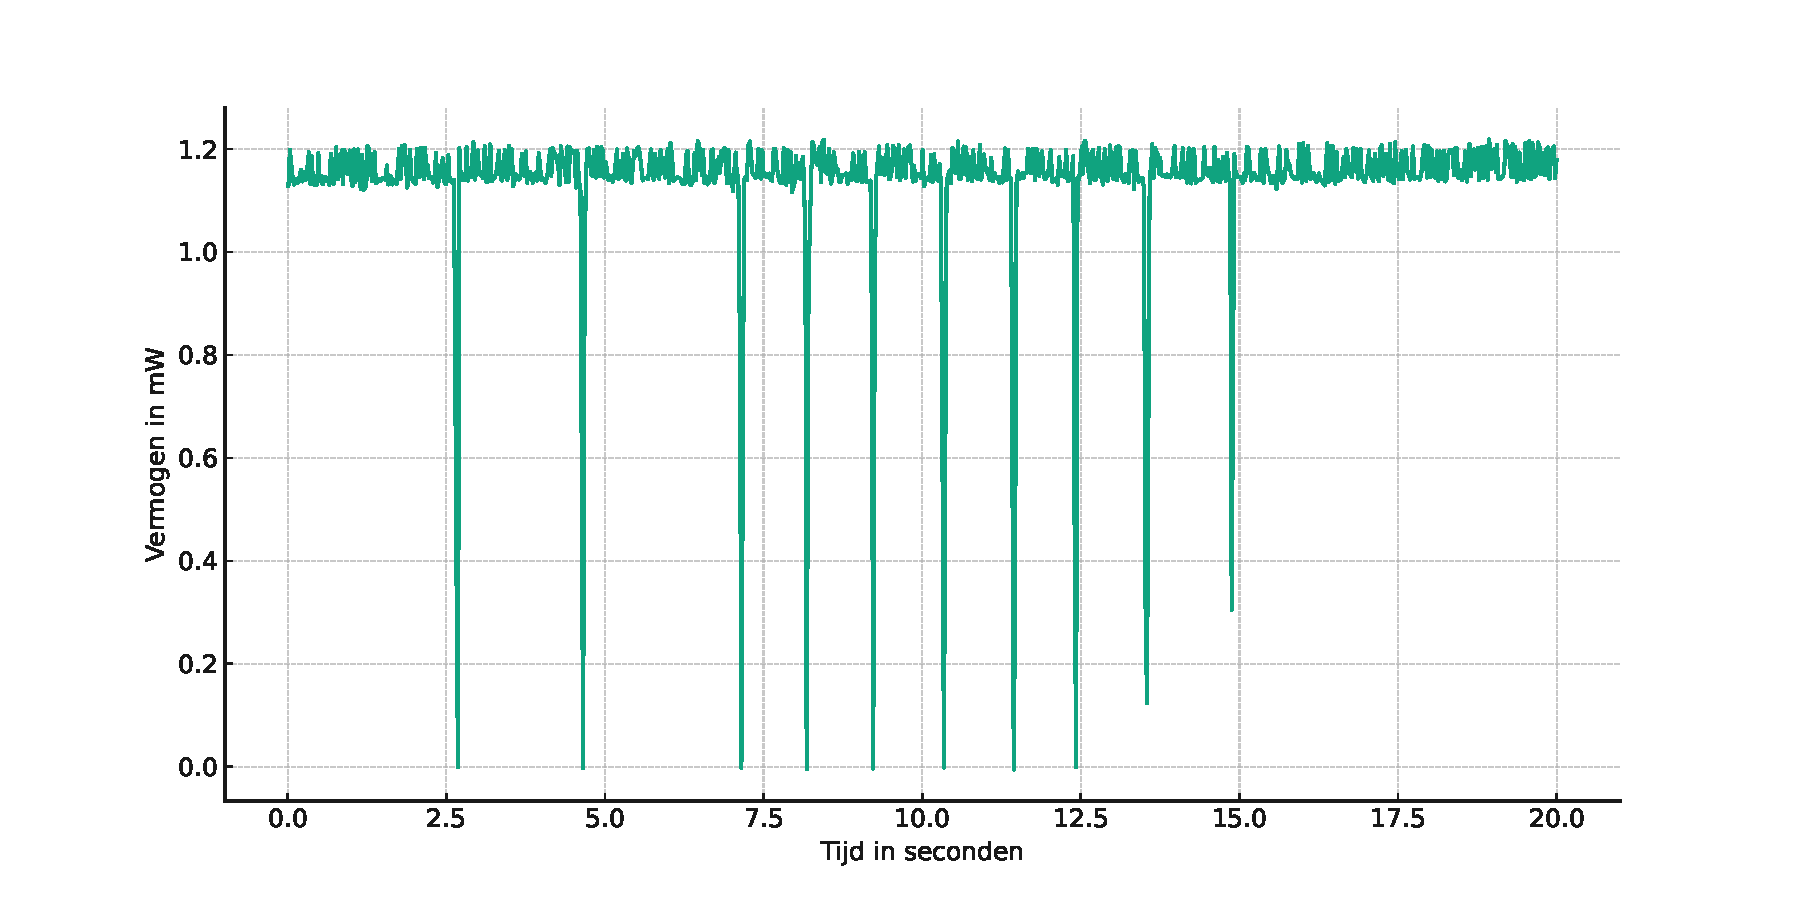
\includegraphics[width=\textwidth]{vermogen_tijd_plot.pdf}
    \caption{Vermogen meting energy harvesting}
    \label{fig:vermogenPlot}
\end{figure}

\subsubsection{Discussie van de energy harvesting test}
In \cref{fig:vermogenPlot} is te zien dat het energieverbruik van de accu naar \qty{0}{\milli\watt} gaat zodra het piëzo element genoeg vibreert. Dit toont aan dat de energy harvesting werkt en de levensduur van de sensormodule zal verlengen.